\section{Design} \label{sec:base}
First we introduce a base design that is extended later on.  Our aim is to hold
CAs accountable in a setting where some, but not all, CT logs are dishonest.  In
other words, the starting-point is to catch misbehaving CAs by adding resilience
against misbehaving CT logs.  The basic idea is shown in
Figure~\ref{fig:design-ca} as three distinct phases:
	a \emph{submission phase} where SFOs are presented to Tor Browser
		and submitted probabilistically to CTRs,
	a \emph{storage phase} where the submitted SFOs are stored for some time to
		obfuscate real-time browsing patterns, and
	an \emph{auditing phase} where the stored SFOs are audited further by adding
		the underlying certificate chains to independent CT logs.
The exact behavior of these phases are governed by parameters set in the Tor
consensus.

\begin{figure*}
	\centering
	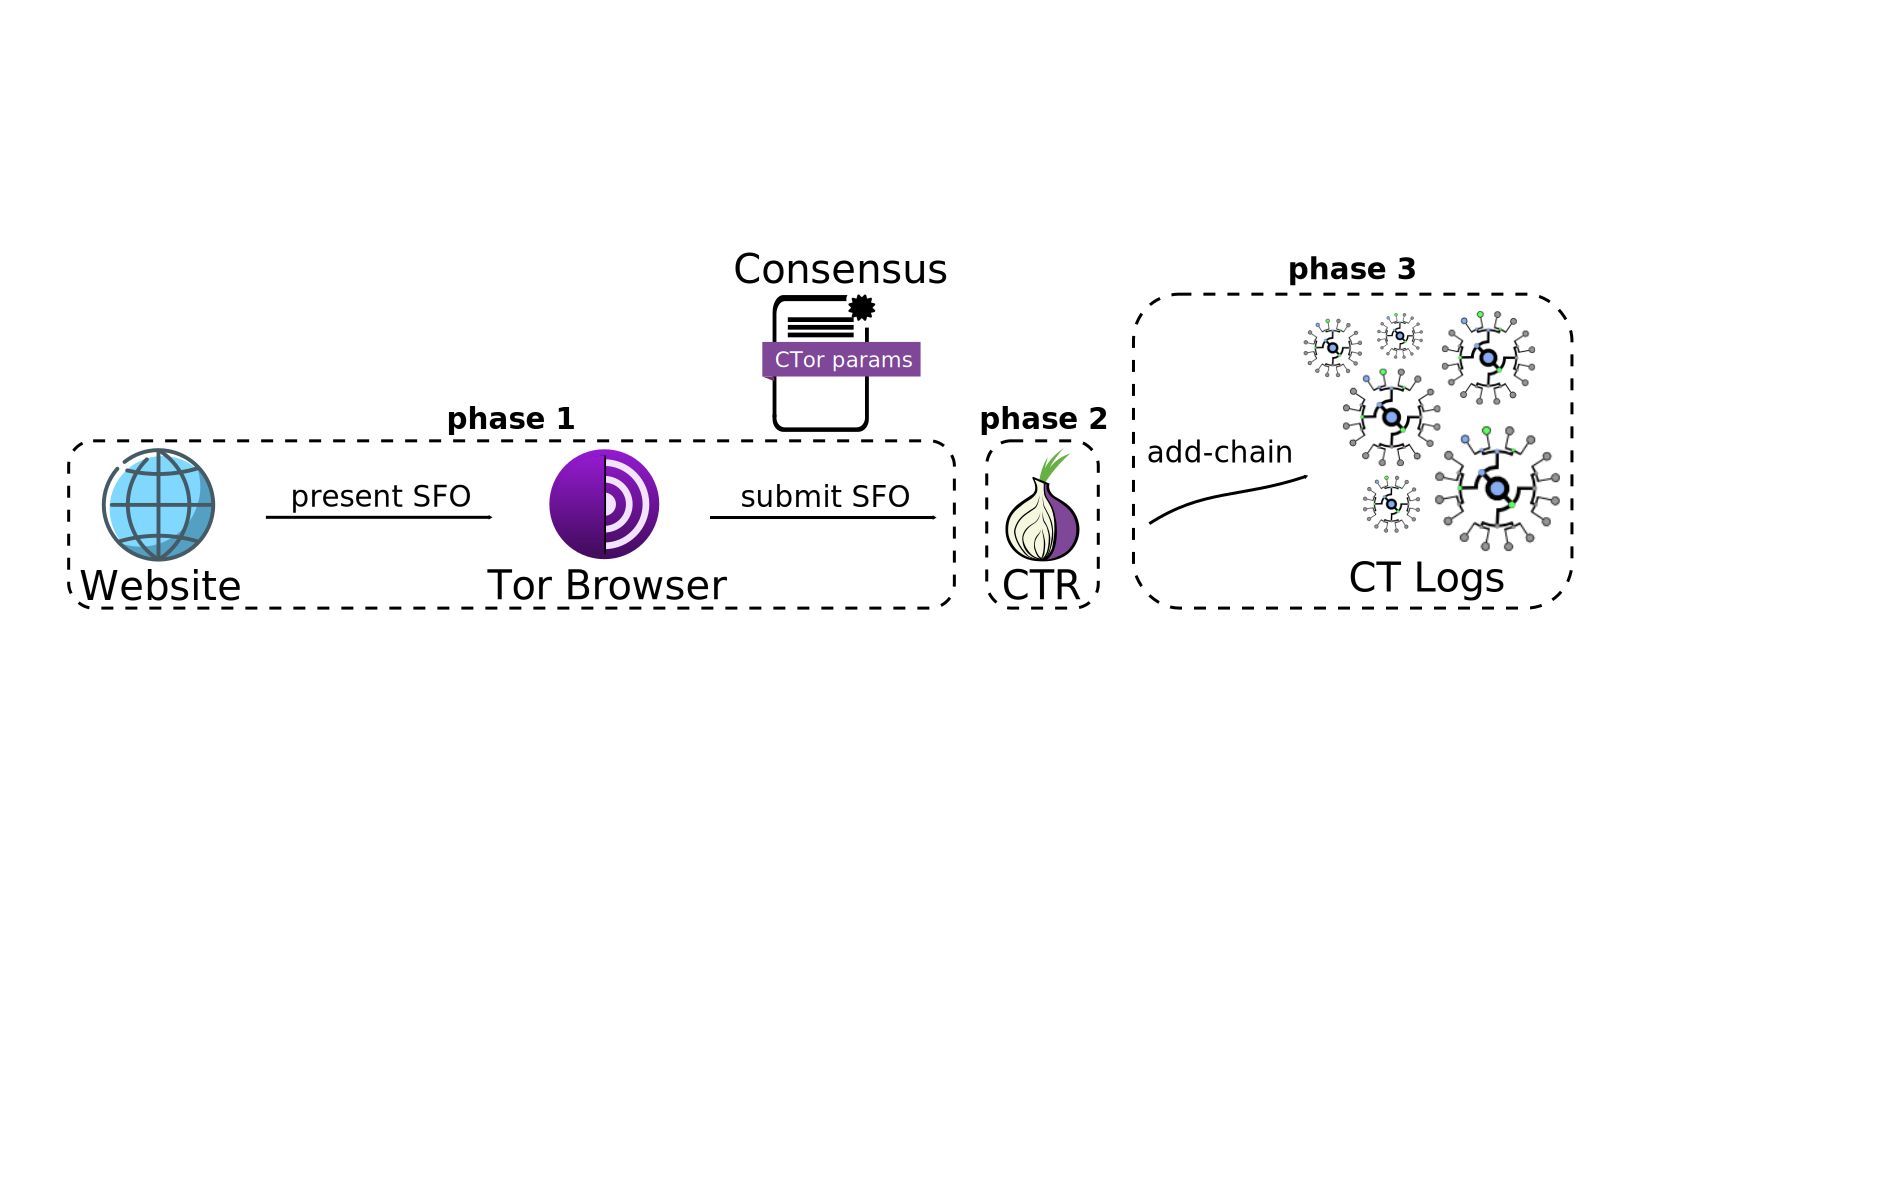
\includegraphics[width=0.85\textwidth]{img/design-ca}
	\caption{%
		The base design of CTor divided into three phases. A website presents an
		SFO to Tor Browser, and Tor Browser in turn with some probability
		submits the SFO to a random CTR (phase 1). A CTR stores the SFO a period
		of time (phase 2). The CTR adds the certificate in the SFO to a random
		independent CT log (phase 3).
	}
	\label{fig:design-ca}
\end{figure*}

\subsection{Tor Consensus} \label{sec:base:consensus}
Our proposal extends Tor's consensus document
so that it entails information regarding
	CTRs,
	recognized CT logs, and
	other necessary parameters that can be tuned.

\subsubsection{CTR Flag} \label{sec:base:consensus:ctr-flag}
The existing \texttt{known-flags} item determines the different flags that a 
given consensus document might contain.  We add another flag named \texttt{CTR},
which indicates that a relay should support CT-auditing as described in
Sections~\ref{sec:base:phase2}--\ref{sec:base:phase3}.  A relay qualifies as a
CTR if it is flagged as \texttt{stable} and \texttt{middle}, which means that we
suggest using resources that are more abundant when compared to, for example,
exit bandwidth.  A Tor relay is assigned the \texttt{CTR} flag if a majority of
directory authorities voted~for~it.

\subsubsection{Recognized CT Log} \label{sec:base:consensus:log}
CTRs only interact with CT logs that are recognized by the Tor consensus.  A log
is recognized if a majority of directory authorities voted for its inclusion by
proposing a \texttt{ct-log-info} entry that contains a log ID, a public key, and
a base URL~\cite{ct,ct/bis}. 
Following from our basic CTR design, there need not be any overlap between the
logs that the Tor consensus recognizes when compared to Tor Browser's CT policy.
There could be overlap, however.  The ideal scenario is that there are many
independent logs that accept certificate chains for most trust anchors.

For now, we do not provide any details as to how the Tor consensus captures
whether two logs are independent or which trust anchors they accept.
Section~\ref{sec:discussion:logs} discusses this and other related
considerations further.

\subsubsection{Other Parameters} \label{sec:base:consensus:params}
Directory authorities influence the way in which Tor Browser and CTRs behave by
voting on other necessary parameters.  For example, the likelihood that
an SFO is submitted to a CTR is a security parameter that is determined by the
value of \texttt{ct-submit-pr}.  Below, the value of an item is computed as the
median of all votes.
\begin{description}
	\item[ct-submit-pr:] A floating-point in $[0,1]$ that determines Tor
		Browser's submission probability.  For example, $0$ disables submission
		while $0.10$ means that every 10$^{\mathsf{th}}$ SFO is sent to a
		random CTR on average.
	\item[ct-sfo-max-bytes:] A natural number that determines how many
		wire-bytes a normal SFO should not exceed.  As outlined in
		Section~\ref{sec:base:phase1}, excessively large SFOs are subject
		to stricter verification criteria.
	\item[ct-log-timeout:] A natural number that determines how long a CTR
		waits before concluding that a CT log is unresponsive, e.g., 10~seconds.
		As outlined in Section~\ref{sec:base:phase3}, timeouts trigger implicit
		resubmissions.
	\item[ct-delay-dist] A distribution that determines how long a CTR should
		wait at minimum before auditing a submitted SFO.  As outlined in
		Section~\ref{sec:base:phase2}, random noise is added to obfuscate
		real-time browsing patterns, e.g., in the order of a few minutes to an
		hour.
	\item[ct-backoff-dist:]
		A distribution that determines how long a CTR should wait between two
		auditing instances, e.g., a few minutes on average.  As outlined in
		Section~\ref{sec:base:phase3}, CTRs audit pending SFOs in batches at
		random time intervals to spread out log overhead.
\end{description}

\subsection{Phase~1---Tor Browser} \label{sec:base:phase1}
The first phase evolves around Tor Browser and how an SFO is validated in the
TLS handshake.  We rely on Tor Browser's trust store to check certificate
chains, an assumed SCT-centric CT policy similar to Chrome~\cite{chrome-policy}
and Safari~\cite{safari-policy} to avoid breakage, and \texttt{ct-max-sfo-bytes}
as well as \texttt{ct-submit-pr} to determine whether and how there should be
any follow-up auditing that goes beyond SCT signature verification.  Given an
incoming SFO $s$:

\begin{enumerate}
	\item Raise a certificate error and stop if the certificate chain of $s$
		is not rooted in Tor Browser's trust store.
	\item Raise a certificate transparency error and stop if the SCTs of $s$
		fail Tor Browser's SCT-centric CT policy.
	\item Accept $s$ and conduct the remaining steps in the background if
		$\mathsf{len}(s) \le \texttt{ct-max-sfo-bytes}$, i.e., without blocking
		the TLS handshake.  Else, wait until the remaining steps are completed
		before accepting $s$.
	\item Flip a biased coin based on \texttt{ct-submit-pr} and stop if the
		outcome indicates no further auditing.
	\item Submit $s$ to a sampled CTR's SFO-endpoint on a pre-built CT-circuit
		that starts from the client's guard and ends at the CTR: three hops in
		total.  The circuit used for submission is closed immediately after
		use without waiting for any acknowledgment.
\end{enumerate}

In other words, an SFO is accepted as valid if the end-entity certificate is
rooted in a trust anchor \emph{and} it has enough SCTs as dictated by an
SCT-centric CT policy.  The decision and possible submission of an SFO to a
random CTR should never block the TLS handshake under normal circumstances,
whereas \emph{excessively large} SFOs do due to high security risks.  See
Section~\ref{sec:analysis:pr:phase1}, which also motivates why it is paramount
that submission circuits are pre-built and closed as soon as possible.

%
% - close circuit asap to make it harder for an attacker to figure out which
% CTR received a submission (should it have access to a zero-day takeover).
% - clearly a submission circuit cannot be reused across tabs, but not doing
% so within tabs may (i) reduce the chance that the receiving CTR knows exactly
% which website was visited, and (ii) make sense because with small submission
% pr (<=1/10) it should be common to submit at most once per tab anyway.
%

\subsection{Phase 2---CTR Storage} \label{sec:base:phase2}
We suggest that CTRs accept SFO submissions on an HTTP endpoint.\footnote{%
	Tor's HTTP DirServer codebase can be reused as extension point to interact
	with the tor daemon, i.e., add another listener.
} For example, Nordberg~\emph{et~al.} defined an SCT feedback interface that can
be reused if an array-length of one is enforced by the CTR~\cite{nordberg}.
With regards to some circuit, process an incoming SFO $s$ as follows:
\begin{enumerate}
	\item\label{enm:ctr-api:close} Close the incoming circuit.
	\item\label{enm:ctr-api:unrecognized} Stop if no CT log in the Tor consensus
		accepts the underlying certificate chain of $s$.
	\item\label{enm:ctr-api:cached}
		Stop if $s$ is cached or pending to be audited already.
	\item\label{enm:ctr-api:audit-after} Compute an \texttt{audit\_after}
		timestamp $\textrm{t} \gets \mathsf{now()} +
			\mathsf{random\_delay}(\texttt{ct-delay-dist})$.
		The former returns the current time and the latter a random delay.
	\item\label{enm:ctr-api:store}
		Add $s$ and its \texttt{audit\_after} timestamp to a buffer of
		pending SFOs that is managed by tor's OOM.
\end{enumerate}

Recall that Tor Browser does not wait for any acknowledgment, and that a
CT-circuit must not be used more than once.  As such, the first step is to
close the incoming circuit once an SFO is received.  The received SFO is
simply discarded if it
	cannot be audited as proposed in Section~\ref{sec:base:phase3},
	is already audited as noted by a cache, or
	is pending to be audited in a buffer of pending SFOs.
For example, the cache could be a collection of SFO hashes and the buffer
something similar to how OOM manages DNS.  A new SFO is stored in the CTR's
buffer alongside an \texttt{audit\_after} timestamp, which specifies the
earliest point in time that the SFO will be audited.  This behavior, where a
random delay is added to each SFO, transforms the CTR into a timed mix such that
less real-time information is leaked to the CT logs in
Section~\ref{sec:base:phase3}.

If memory becomes a scarce relay resource, e.g., due to flooding, OOM
should delete SFOs at random~\cite{nordberg}.  The threat of flooding is
discussed further in Section~\ref{sec:analysis}.

\subsection{Phase 3---Auditing} \label{sec:base:phase3}
CTR auditing is initiated at random time intervals to spread out the load
imposed by the Tor network on CT logs.  Each auditing instance is composed of
circuit setup, a core loop of SFO enumeration, and circuit tear-down.

\begin{enumerate}
	\item\label{enm:ctr:audit:backoff} Sample a uniform delay from
			$[0, \texttt{ct-backoff}]$,
		then schedule a timer and wait until that time elapsed.
	\item\label{enm:ctr:audit:log-circuit} Establish a new circuit and use it
		for all subsequent log connections.  Connect to the logs when needed.
	\item\label{enm:ctr:audit:loop} Enumerate the buffer of pending SFOs:
		\begin{enumerate}
			\item\label{enm:ctr:audit:too-soon} Continue the loop if
				$\textrm{SFO}.\mathsf{audit\_after} > \mathsf{now}()$.
			\item\label{enm:ctr:audit:sample}
				Sample a log uniformly at random that accepts the underlying
				certificate chain $c \in s$.  Do not consider any log that the
				SCTs of $s$ refer if the Tor consensus lists any independent
				log.\footnote{%
					TODO: needs to be expressed better.  The point is that we
					want to prioritize adding the certificate chain to an
					independent log that the attacker does not control.
				}
			\item\label{enm:ctr:audit:log} Use \texttt{ct-query-timeout} to set
				a timer and submit $c$ for public logging to the log's
				\texttt{add-chain}~\cite{ct} or
				\texttt{submit-entry}~\cite{ct/bis} endpoint.
				\begin{itemize}
					\item\label{enm:ctr:audit:log:success} On valid
						SCT: cache the SFO, then discard it from the buffer of
						pending SFOs.
					\item\label{enm:ctr:audit:log:fail} On any other outcome:
						break the loop.
				\end{itemize}
		\end{enumerate}
	\item\label{enm:ctr:audit:teardown} Close all opened circuits and go back to
		step~\ref{enm:ctr:audit:backoff}.
\end{enumerate}

As shown above we take an unusual approach towards auditing SFOs.  Rather than
following up on an SCT's inclusion status, we submit the underlying
certificate chain to an independent CT log.  As such, the end-entity certificate
will make it into the public domain if the sampled log is not controlled by the
attacker.  If there is no independent log listed in the Tor consensus, it is
still valuable to resubmit to a dependent log:
	it might be the case that the attacker has access to a log's signing key,
	but not the log's actual infrastructure.
In other words, a mis-issued certificate would make it into the public domain in
such a scenario if we resubmit it rather than discarding it due to lack of
an independent log.

After a certificate chain is submitted for logging, the returned SCT must be
valid, e.g., correct structure and signed by the log in question.  On any other
outcome, such as a timeout, the SFO remains in the buffer of pending SFOs while
the CTR goes into back-off mode.

% TODO: should we fixate so that resubmission to the same sampled log?
% TODO: is it really motivated to "break" now rather than "continue"?
